% --- SEZIONE 1: COMPONENTI DI SISTEMA E CONTROLLO ---

\section{Componenti del Sistema (SCS)}
Il \textbf{System Control Space (SCS)} gestisce le funzionalità core del processore, inclusa la configurazione del NVIC e del registro di controllo di sistema.

\subsection{Meccanismi di Fault e Eccezioni}
\begin{itemize}
    \item \textbf{HardFaults:} Sempre attivati; gestiscono errori di Bus, Usage e Memory Management. Permettono una reazione rapida agli errori critici.
    \item \textbf{Wake-up Interrupt:} Consente la disattivazione gerarchica dei componenti
     per ridurre il consumo energetico (modalità Sleep/Stop).
    \item \textbf{Memory Protection Unit (MPU):} Genera eccezioni in caso di accessi non autorizzati alla memoria.
    \item \textbf{Debug Unit:} Fornisce fino a 4 breakpoint hardware per il debugging del codice.
\end{itemize}

\subsection{System Tick Timer (SysTick)}
Un contatore a \textbf{24-bit} che fornisce una base dei tempi costante per il sistema operativo o i cicli di programma.


\section{Gestione degli Interrupt (NVIC)}

\begin{itemize}
    \item Il \textbf{Nested Vector Interrupt Controller} gestisce la prioritizzazione e
     il passaggio tra il programma di background e le 
     \textbf{Interrupt Service Routine (ISR)}.
    \item L'LSB in ogni vettore indica la modalità di salto (1: thumb, 0: ARM) nei Cortex-M sempre 1
    \item Solitamente la VT (vector table) viene slavata in memoria fra il boot code e la seconda istruzione
    \item Tramite VTOR (vetor table Offset Register) è possible cambaire la posizione
\end{itemize}



\begin{minipage}[b]{0.51\columnwidth}
    \subsection{Registri di Mascheramento}
    \begin{itemize}
        \item \textbf{PRIMASK:} 1 bit per disabilitare tutti gli interrupt (tranne HardFault e NMI).
        \item \textbf{FAULTMASK:} 1 bit per disabilitare interrupt e tutte le eccezioni.
        \item \textbf{BASEPRI:} Disabilita interrupt con priorità inferiore a un valore impostato.
    \end{itemize}
    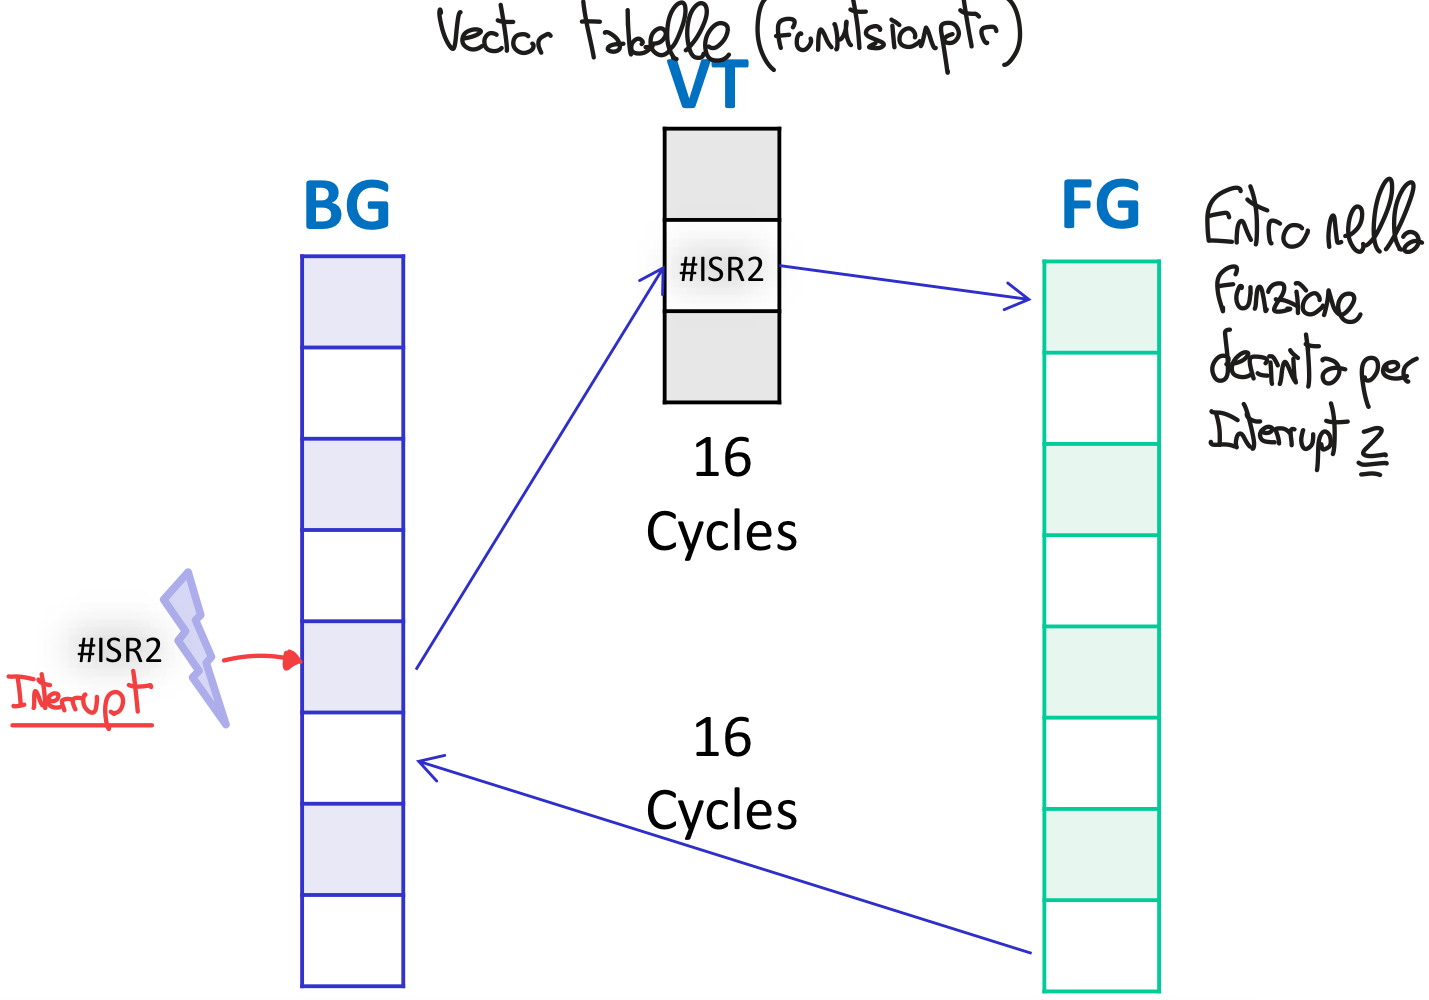
\includegraphics[width=\linewidth]{images/NVIC_sequence.png}
\end{minipage}
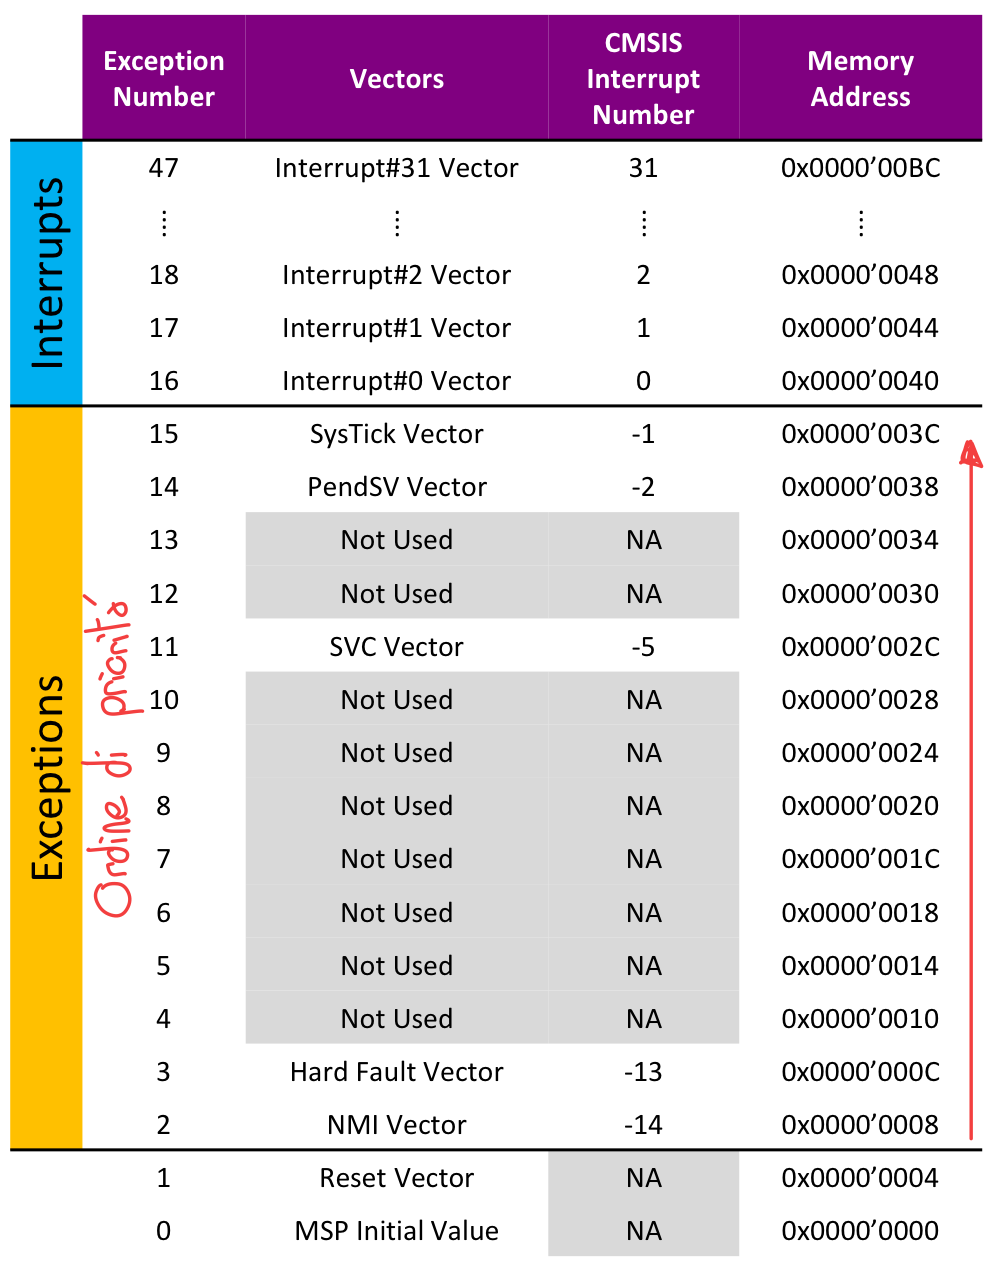
\includegraphics[width=0.49\columnwidth]{images/NVIC_table.png}

% --- SEZIONE 2: MODELLO DI MEMORIA E STACK ---

\section{Stack e Gestione Memoria}
Lo \textbf{Stack} è una memoria temporanea utilizzata per variabili locali e salvataggio contestuale durante le eccezioni.
\begin{itemize}
    \item \textbf{Direzione:} Cresce verso indirizzi di memoria inferiori.
    \item \textbf{Stack Pointer (SP):} Punta sempre al "top of stack". È vietato leggere o scrivere al di sotto di SP.
    \item \textbf{Allineamento:} Normalmente allocato in step di 8 byte.
    \item \textbf{Velocità:} L'accesso allo stack è circa due volte più rapido del RAM/ROM pointer poiché l'indirizzo (SP) è già disponibile.
\end{itemize}

\subsection{Estensioni e Manipolazione}
\begin{itemize}
    \item \textbf{SXTB/UXTH:} Estensione del segno o zero-fill (4 byte $\leftarrow$ 1/2 byte).
    \item \textbf{REV/REV16:} Inversione dell'ordine dei byte (Endianness conversion).
    \item \textbf{CMP/CMN:} Confronti che aggiornano le flag senza salvare il risultato (es. \texttt{CMP} esegue \texttt{SUBS}).
\end{itemize}

% --- SEZIONE 3: ARCHITETTURE E COMPILAZIONE ---

\section{Confronto Architetture ARM Cortex}
La famiglia Cortex si divide in tre profili ottimizzati per diversi scenari:
\begin{description}
    \item[Cortex-A (Application):] Calcolo generico ad alte prestazioni (Linux/Android).
    \item[Cortex-R (Real-Time):] Bassa latenza e alta affidabilità (automotive/medico).
    \item[Cortex-M (Microcontroller):] Ridotto consumo energetico, interrupt deterministici.
\end{description}

\renewcommand{\arraystretch}{1.5}
\resizebox{\columnwidth}{!}{
\begin{tabular}{|l|c|c|c|c|c|c|c|c|}
\hline
\textbf{Core} & \textbf{Thumb} & \textbf{Thumb-2} & \textbf{HW Mult.} & \textbf{HW Div.} & \textbf{Math Sat.} & \textbf{DSP} & \textbf{FPU} & \textbf{Arch} \\
\hline
Cortex-M0  & \cellcolor{green!60}Mostly & \cellcolor{green!60}Subset & \cellcolor{green!60}1/32 cyc & \cellcolor{red!60}No & \cellcolor{red!60}No & \cellcolor{red!60}No & \cellcolor{red!60}No & ARMv6-M \\
Cortex-M0+ & \cellcolor{green!60}Mostly & \cellcolor{green!60}Subset & \cellcolor{green!60}1/32 cyc & \cellcolor{red!60}No & \cellcolor{red!60}No & \cellcolor{red!60}No & \cellcolor{red!60}No & ARMv6-M \\
Cortex-M1  & \cellcolor{green!60}Mostly & \cellcolor{green!60}Subset & \cellcolor{green!60}3/33 cyc & \cellcolor{red!60}No & \cellcolor{red!60}No & \cellcolor{red!60}No & \cellcolor{red!60}No & ARMv6-M \\
Cortex-M3  & \cellcolor{green!60}Fully  & \cellcolor{green!60}Fully  & \cellcolor{green!60}1 cyc    & \cellcolor{green!60}Yes & \cellcolor{green!60}Yes & \cellcolor{red!60}No  & \cellcolor{red!60}No & ARMv7-M \\
Cortex-M4  & \cellcolor{green!60}Fully  & \cellcolor{green!60}Fully  & \cellcolor{green!60}1 cyc    & \cellcolor{green!60}Yes & \cellcolor{green!60}Yes & \cellcolor{green!60}Yes & \cellcolor{yellow!60}Optional & ARMv7E-M \\
Cortex-M7  & \cellcolor{green!60}Fully  & \cellcolor{green!60}Fully  & \cellcolor{green!60}1 cyc    & \cellcolor{green!60}Yes & \cellcolor{green!60}Yes & \cellcolor{green!60}Yes & \cellcolor{yellow!60}Optional & ARMv7E-M \\
\hline
\end{tabular}}
\renewcommand{\arraystretch}{1}

\subsection{Evoluzione Cortex-M0 vs M0+}
\begin{itemize}
    \item \textbf{M0+ Pipeline:} Ridotta a 2 stadi per maggiore efficienza.
    \item \textbf{Accesso I/O:} Supporto per Single-Cycle GPIO.
    \item \textbf{Debugging:} Micro Trace Buffer (MTB) opzionale per il tracciamento dei salti.
    \item \textbf{MPU}
\end{itemize}

\subsubsection{Pipeline}
\begin{itemize}
    \item[+] Es wird in jedem Cycle ein Befehl ausgeführt
    \item [-] Bei sprüngen muss die Pipeline 'geleert' werden
\end{itemize}

\section{Adressierungsarten ARM (Cortex-M0)}
\begin{itemize}
    \item Register direkt
    \item Register Indirekt
    \item Register Indirekt mit offset \texttt{[R?, \#imm]}
    \item Register Indirekt mit index \texttt{[R?, R?]}
\end{itemize}

\subsection{Register Direkt, Immediate}
\begin{itemize}
    \item \textbf{Immediate:} \texttt{MOV R0, \#100} $\rightarrow$ Valore caricato direttamente.
    \item \textbf{Register:} \texttt{MOVS R2, R1} $\rightarrow$ Copia valore tra registri.
    \item \textbf{Limitazioni:} Gli immediati sono codificati nell'istruzione (es. 8-bit per \texttt{MOVS}).
\end{itemize}
x
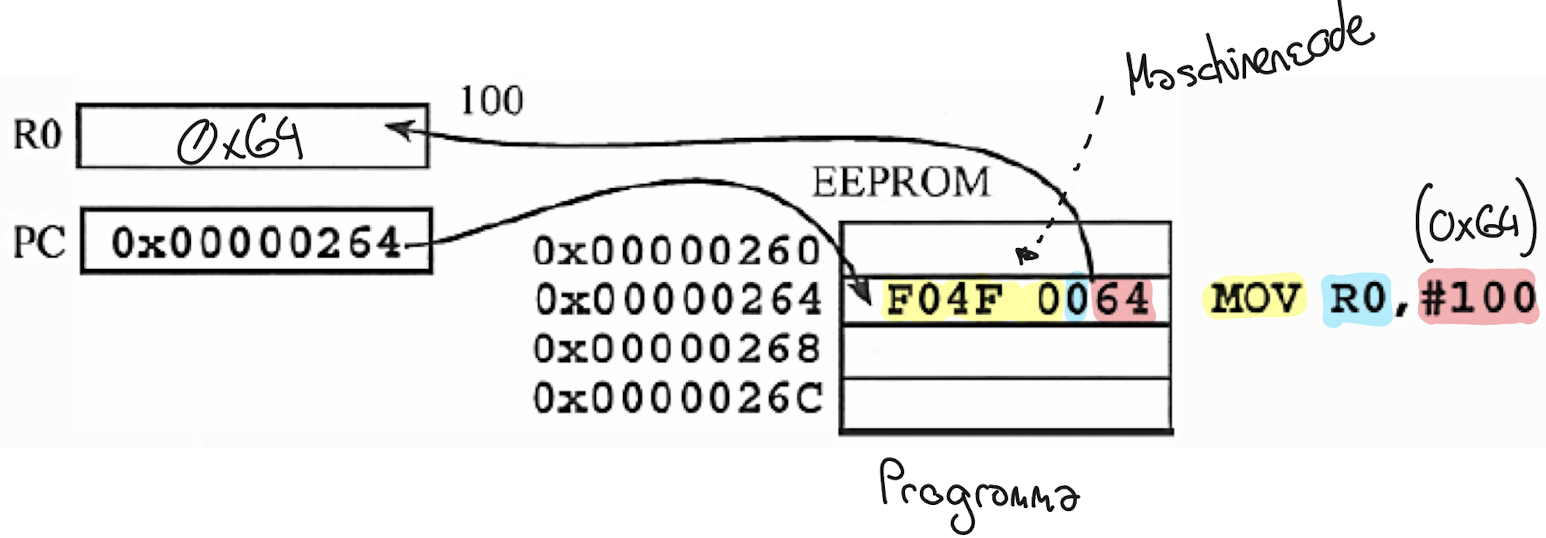
\includegraphics[width=\columnwidth]{images/register_direkt.png}

\subsection{Register Indirekt (ptr)}
\begin{itemize}
    \item \textbf{Semplice:} \texttt{LDR R0, [R1]} \\
    $\rightarrow$ $R0 = \text{valore all'indirizzo } R1$.
    \item \textbf{Con Offset:} \texttt{LDR R0, [R1, \#4]} $\rightarrow$ $R0 = \text{valore all'indirizzo } R1 + 4$ (utile per array/struct).
    \item \textbf{Con Index:} \texttt{LDR R0, [R1, R2]} \\
    $\rightarrow$ $R0 = \text{valore all'indirizzo } R1 + R2$.
\end{itemize}    
\begin{center}
    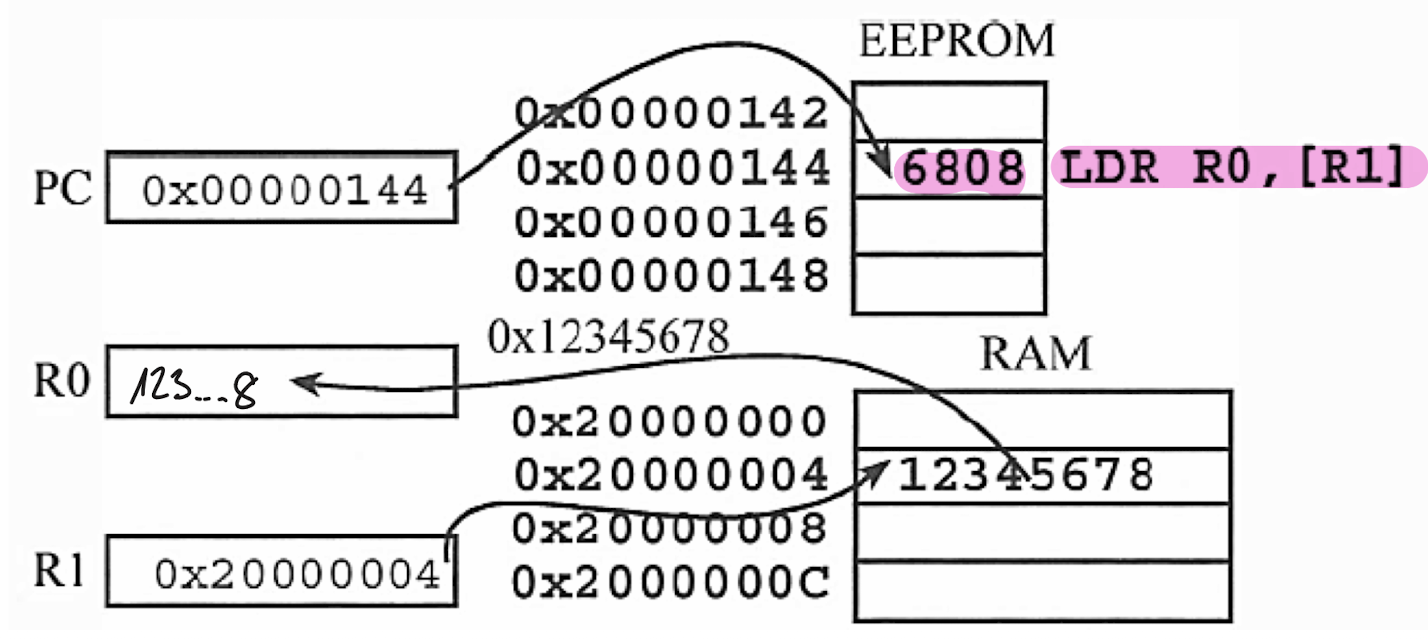
\includegraphics[width=0.7\columnwidth]{images/register_indirekt.png}
\end{center}

\subsection{PC-Relative \& Literal Pool}
\begin{itemize}
    \item \textbf{Problema:} Istruzioni da 32-bit non possono contenere costanti da 32-bit.
    \item \textbf{Soluzione:} L'assembler salva la costante nel \textbf{Literal Pool} (zona memoria vicina).
    \item \textbf{Accesso:} \texttt{LDR R0, =0x12345678} viene tradotto in \texttt{LDR R0, [PC, \#offset]}.
    \item Richiedono sempre \textbf{due accessi} alla memoria
\end{itemize}

\subsection{Registerlisten \& Stack (SP-Relative)}
\begin{itemize}
    \item \textbf{Multiple:} \texttt{LDM R7!, \{R0-R3, R5\}} $\rightarrow$ Carica più registri partendo da indirizzo in $R7$.
    \item \textbf{Stack:} \texttt{PUSH \{R0-R2\}}, \texttt{POP \{R0-R2\}}.
    \item \textbf{Regola d'oro:} Il registro con numero più basso (\texttt{R0}) va sempre all'indirizzo di memoria più basso. L'ordine nelle graffe non conta per l'hardware.
\end{itemize}

\subsection*{Stack Framing}
Lo Stack Frame è lo spazio riservato nella RAM per le variabili locali di una funzione.

\begin{minipage}{0.5\columnwidth}
    \begin{itemize}
        \item \textbf{Allocazione:} \texttt{SUB SP, SP, \#X} riserva $X$ byte (lo stack cresce verso indirizzi bassi).
        \item \textbf{Frame Pointer ($R7$):} Si usa \texttt{MOV R7, SP} per avere un riferimento fisso all'inizio del frame.
        \item \textbf{Accesso:} Le variabili vengono scritte/lette usando offset rispetto a $R7$, es: \texttt{STR R0, [R7, \#4]}.
        \item \textbf{Deallocazione:} Prima del ritorno (\texttt{BX LR}), si deve pulire lo stack con \texttt{ADD SP, SP, \#X}.
    \end{itemize}
\end{minipage}
\begin{minipage}{0.5\columnwidth}
    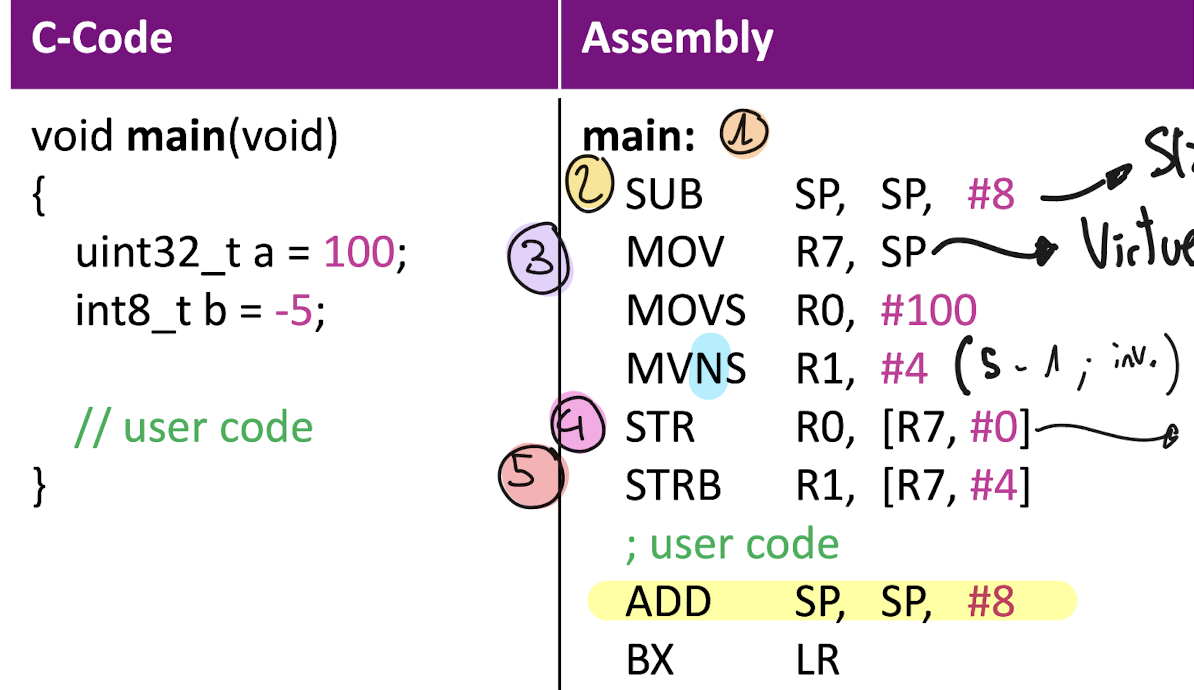
\includegraphics[width=\linewidth]{images/stack_framing.png}
\end{minipage}

\section{Il Processo di Compilazione}
Il codice sorgente viene trasformato in binario attraverso diverse fasi:

\begin{enumerate}
    \item \textbf{Preprocessore:} Gestisce inclusioni e macro. (\texttt{\#define}, \texttt{\#if}, \dots)
    \item \textbf{Compilatore:} Traduce il linguaggio ad alto livello in Assembly.
    \item \textbf{Assembler:} Converte Assembly in codice macchina rilocabile.
    \item \textbf{Linker/Binder:} Unisce file oggetto e librerie.
    \item \textbf{Loader:} Converte indirizzi rilocabili in assoluti e carica in memoria.
\end{enumerate}

\subsection{Analisi del Compilatore}
\begin{itemize}
    \item \textbf{Analisi Lessicale:} Rimozione spazi e raggruppamento token.
    \item \textbf{Analisi Sintattica/Semantica:} Controllo struttura e tipi di dati.
    \item \textbf{Ottimizzazione:} Miglioramento del codice per velocità o spazio.
    \item \textbf{Generazione:} Produzione del codice target.
\end{itemize}

\section{Interfacciamento I/O}
Le periferiche sono mappate in memoria (\textit{Memory Mapped I/O}) tramite registri specifici:
\begin{itemize}
    \item \textbf{Datenregister:} Contiene i dati da elaborare.
    \item \textbf{Steuerregister:} Configurazione della periferica.
    \item \textbf{Statusregister:} Indica lo stato corrente dell'I/O (es. Busy, Ready).
\end{itemize}


\section{Esempi}\vspace{-0.3em}
\lstinputlisting[style=armasmstyle]{code/64_bit_addition.s}\vspace{-0.6em}
\lstinputlisting[style=armasmstyle]{code/64_bit_subtraction.s}\vspace{-0em}

\begin{minipage}{0.7\columnwidth}
    \lstinputlisting[style=armasmstyle]{code/64_bit_shift.s}
\end{minipage}
\begin{minipage}{0.3\columnwidth}
    \centering
    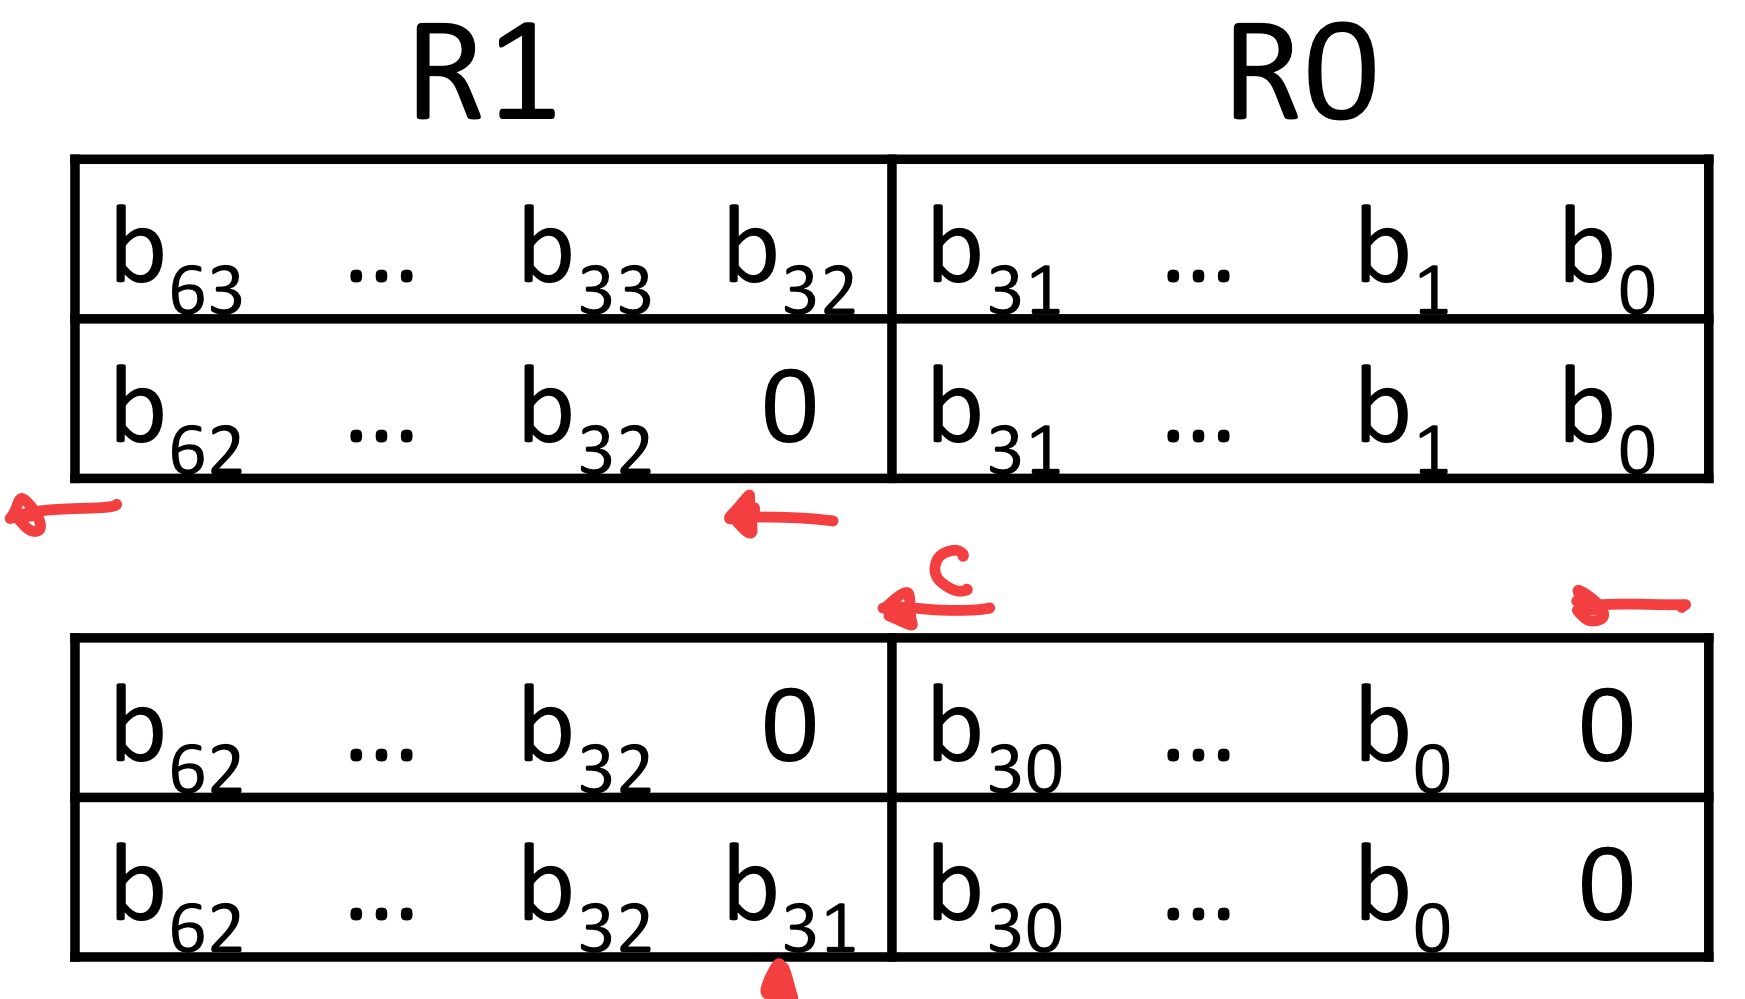
\includegraphics[width=\linewidth]{images/64_bit_shift.png}\medbreak
    Equivalente a: ($\cdot 2$)
\end{minipage}

% --- ESEMPIO 1 ---
\noindent
\begin{minipage}[t]{0.25\columnwidth}
    \vspace{0pt} % Forza l'allineamento in alto
    \centering
    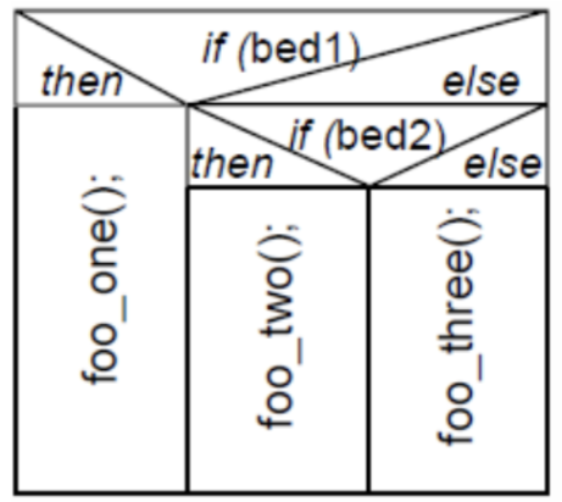
\includegraphics[width=\linewidth]{images/triple_if_else.png}
\end{minipage}% <-- Il % previene spazi orizzontali extra
\hfill
\begin{minipage}[t]{0.72\columnwidth}
    \vspace{0pt}
    \setlength{\fboxsep}{2pt} % Riduce l'altezza del box viola
    
    \begin{minipage}[t]{0.48\textwidth}
        \colorbox{sectioncolor}{\makebox[\dimexpr\linewidth-2\fboxsep\relax]{\footnotesize\textbf{\color{white}Thumb-2 Assembly}}}
        \lstinputlisting[style=armasmstyle, basicstyle=\footnotesize\ttfamily, aboveskip=2pt, belowskip=0pt]{code/beispiel_1.s}
    \end{minipage}%
    \hspace{0.04\textwidth}%
    \begin{minipage}[t]{0.48\textwidth}
        \colorbox{sectioncolor}{\makebox[\dimexpr\linewidth-2\fboxsep\relax]{\color{white}\footnotesize\textbf{C Source Code}}}
        \lstinputlisting[language=C, basicstyle=\footnotesize\ttfamily, aboveskip=1pt, belowskip=0pt]{code/beispiel_1.c}
    \end{minipage}
\end{minipage}

\vspace{1ex} % Spazio ridotto tra i due esempi

% --- ESEMPIO 2 ---
\noindent
\begin{minipage}[t]{0.25\columnwidth}
    \vspace{0pt}
    \centering
    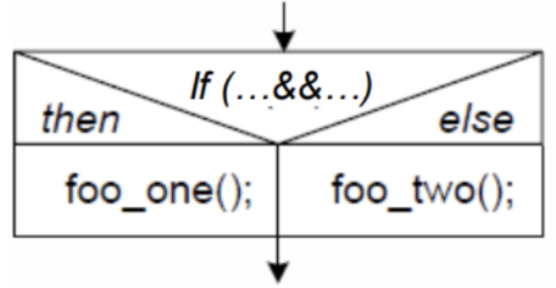
\includegraphics[width=\linewidth]{images/if_else.png}
\end{minipage}%
\hfill
\begin{minipage}[t]{0.72\columnwidth}
    \vspace{0pt}
    \setlength{\fboxsep}{2pt}
    
    \begin{minipage}[t]{0.48\textwidth}
        \colorbox{sectioncolor}{\makebox[\dimexpr\linewidth-2\fboxsep\relax]{\footnotesize\textbf{\color{white}Thumb-2 Assembly}}}
        \lstinputlisting[style=armasmstyle, basicstyle=\footnotesize\ttfamily, aboveskip=2pt, belowskip=0pt]{code/beispiel_2.s}
    \end{minipage}%
    \hspace{0.04\textwidth}%
    \begin{minipage}[t]{0.48\textwidth}
        \colorbox{sectioncolor}{\makebox[\dimexpr\linewidth-2\fboxsep\relax]{\footnotesize\textbf{\color{white}C Source Code}}}
        \lstinputlisting[language=C, basicstyle=\footnotesize\ttfamily, aboveskip=1pt, belowskip=0pt]{code/beispiel_2.c}
    \end{minipage}
\end{minipage}

\begin{center}
    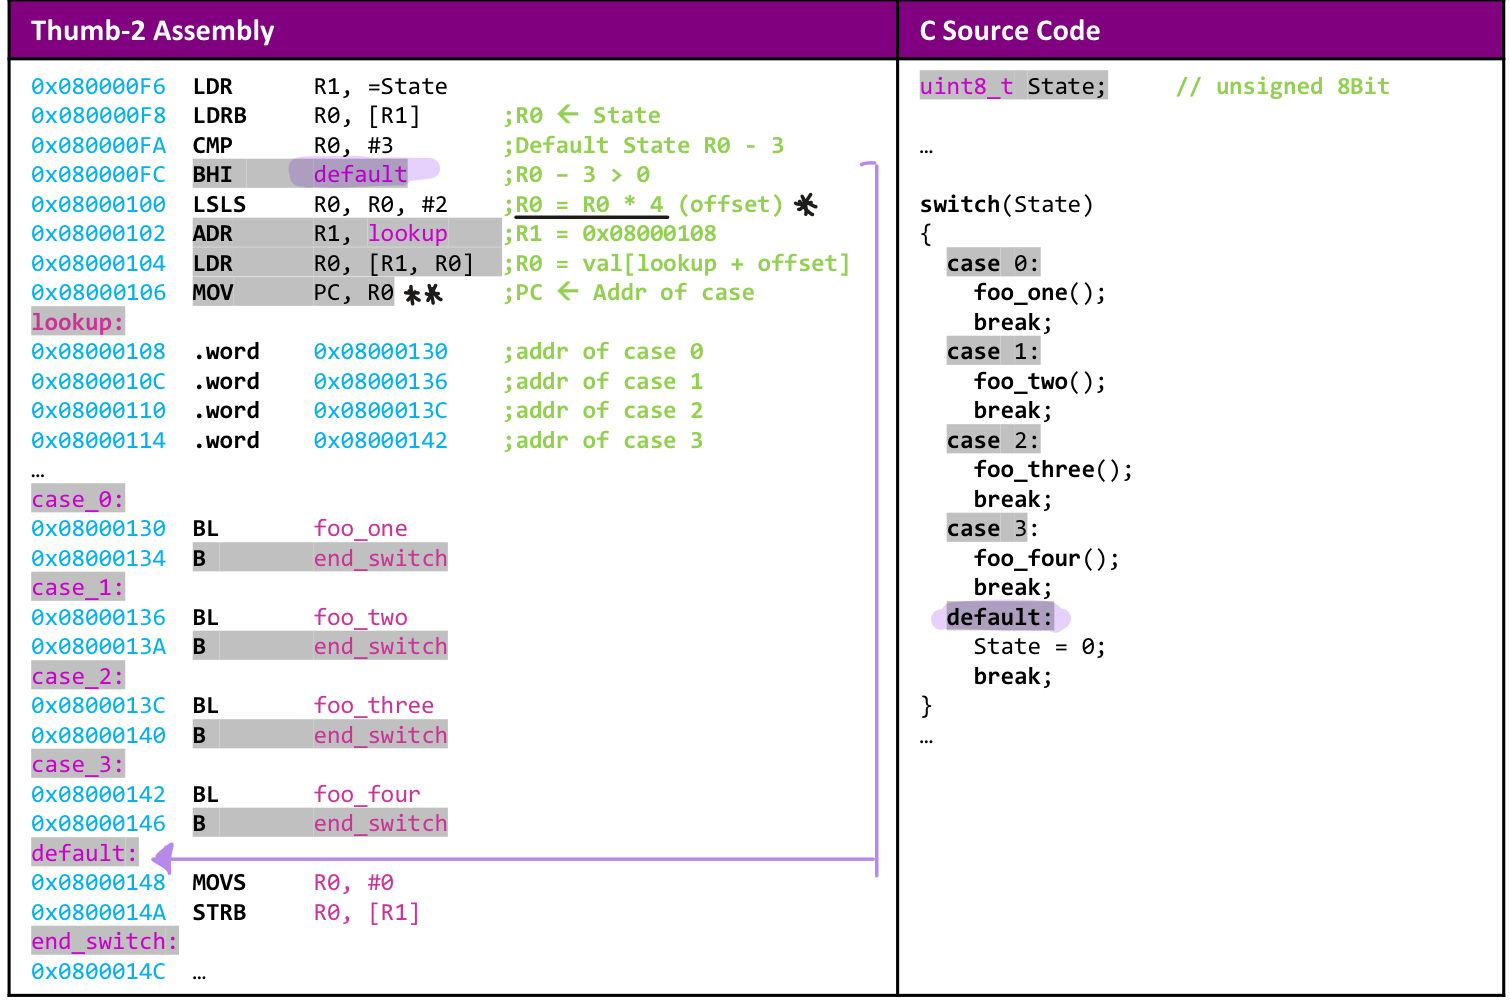
\includegraphics[width=0.9\linewidth]{images/switch_case.png}
\end{center}

\begin{enumerate}
    \item \textbf{Controllo dei limiti (Bound Check):} Verifica iniziale del valore di \texttt{State} per saltare subito al \texttt{default} se l'indice è fuori range.
    \item \textbf{Calcolo dell'offset:} Moltiplicazione del valore per 4 ($State \ll 2$) tramite shift logico, poiché ogni puntatore nella look-up table occupa 32 bit (4 byte).
    \item \textbf{Recupero del puntatore:} Lettura dell'indirizzo di destinazione esatto sommando l'offset calcolato all'indirizzo base della tabella.
    \item \textbf{Salto (Branch):} Caricamento dell'indirizzo recuperato nel Program Counter (\texttt{PC}) per avviare l'esecuzione del caso specifico.
\end{enumerate}

% \lstinputlisting[style=armasmstyle]{code/extension.s}